\section{Introduction}

%Dans le cadre de notre Licence Fondamentale en Sciences de L'informatique à
%la Faculté des Sciences de Sfax, nous avons utilisé nos connaissances pour
%réaliser un projet de fin d'études pendant un stage dans Djagora Academy.
%Ce chapitre présente une mise en contexte et une description de la problématique
%et trace les objectifs de notre projet. De tel projet consiste a réaliser une
%plateforme \FIXME{complete phrase}

Dans cette partie, nous allons présenter l'académie \textquote{Djagora Academy}
au sein duquel nous avons effectué notre stage de fin d'études et le projet
\textquote{CityWatch} que nous sommes en train de réaliser avec la communauté
de l'académie. Nous allons présenter l'objective du projet et la méthodologie de
gestion suivi pour le réaliser.

\subsection{Présentation de l'académie}

Djagora Academy est un programme de mentorat visant accompagner des étudiants
en année terminale dans la réalisation de projets d'intérêt publique dans le but
est la création des startups.

Pendant la réalisation des projets des idées des startups, les étudiants
(mentorés)  seront accompagnés par des universitaires et des industriels
(mentors) avec le soutien de plusieurs compagnies internationales, telles que
l'European Center for Leadership and Entrepreneurship Education (Eclee France,
Eclee USA), Djagora University (SénégaL), NorthStar Paradigm Education (USA),
Continental (Allemagne), Sivantos (Allemagne), Yousoft-IT (Tunisie),
Factory Campus (Tunisie).

%Considérés comme des idées de startups, les projets proposés par le comité de
%pilotage de l'Académie Djagora se substituent aux projets de fin d'études.
%La durée de réalisation d'un projet s'étale sur cinq mois. Cette période
%correspond à un cycle d'accélération de startups. Tout au long de ce cycle,
%les mentorés suivront un programme de formations généralement certifiantes.

%Mis-à-part le programme de mentorat et le cycle d'accélération de startups,
%l'Académie Djagora déclare le défi et organise une compétition tout au long
%du cycle d'accélération de startups. Nommée «Bourse des startups», cette
%compétition unique en son genre, dont l'idée est attribuée à Factory Campus,
%est une bonne opportunité pour tous les intervenants de l'Académie Djagora.
%La «Bourse des startups» vise joindre l'utile du modèle financier et des retombées
%économiques de la bourse et de l'entrepreneuriat en général à l'agréable des
%bonnes pratiques et cultures du défi, de la concurrence, du challenge et du
%leadership.

\subsection{Présentation du sujet}

Le projet consiste en la création d'un système logiciel de collecte, de
traitement, d'analyse, de fouille et de visualisation des données/informations.
Il est décomposé en deux sous systèmes. L'un se charge de la collecte. L'autre,
quant à lui, est chargé du reste; du traitement à la visualisation.
Celui, chargé de la collecte, assimile dans un premier temps à une application
mobile capable de collecter des informations d'une façon automatique en se
basant uniquement sur les capteurs intégrés aux smartphones/tablettes
(mobile sensors), soit encore de façon semi-automatique faisant appel aux
simples intéractions de l'utilisateur (utilisateur citoyen).
Le deuxième sous système assimile à une application web permettant le
traitement, l'analyse syntaxique et sémantique, la fouille des
informations/données collectées pour enfin assurer leur visualisation.

En prenant départ d'un récepteur de position, le sujet mit à résoudre les
problématiques localisations de multiple individu, la réalisation d'un module
d'itinéraire pour les véhicules vers enfin la création d'un mécanisme qui donne
la main à effectuer divers types de rapport dans une carte.

\subsection{objectifs du projet}

L'objective du projet est de former une seule plateforme qui vise une variété
des secteurs. Nous allons maximiser le nombre des types de données collectées à
fin d'avoir un ensemble des informations que nous pouvons les utiliser pour
fournir des servies de consultation et de conseil.

Ces services de consultation peuvent support des différents secteurs incluant
les secteurs de transport, de média, de santé et plusieurs autres secteurs
privés et public.

Nos services ciblent aussi les utilisateurs citoyens comme source très
important d'information. Des services d'intérêt public seront lui fournir.

\subsection{Méthode de gestion de projet utilisée}

\subsubsection{Présentation de la méthode agile SCRUM}

Scrum est une méthode de gestion de projets dans laquelle des équipes
multifonctionnelles réalisent des produits de manière itérative et incrémentale.
Tout au long de cette méthode, le développement est définit, d'une façon
incrémentale, en cycles de travail appelés Sprints. Un sprint est définit sous
la forme d'un certain nombre de tâches à réaliser au cours d'une itération.
Cette dernière ne dure jamais plus que quatre semaines (deux semaines la
plupart du temps). Les itérations s'enchainent l'une après l'autre sans
interruption. Les Sprints se terminent à une date spécifique. Ceux-ci ne
peuvent être prolongés même si le travail ne soit pas terminé. Généralement les équipes
Scrum choisissent une durée de Sprint et la maintiennent durant le projet, jusqu'à ce
qu'elles puissent encore augmenter leur productivité et utiliser alors un cycle plus court.
Au début de chaque Sprint, une équipe multifonctionnelle (environ de quatre à sept
personnes) sélectionne des tâches (exigences du client) dans une liste priorisée.
L'équipe s'accorde collectivement sur une cible constituée de ce qu'elle pense pouvoir
livrer à la fin du Sprint. Aucune nouvelle tâche n'est ajoutée durant le Sprint. Chaque
jour, l'équipe se réunit brièvement afin de contrôler sa progression et ajuster les
prochaines étapes nécessaires à la finalisation du travail restant au sein d'un Sprint. A la
fin de chaque Sprint, une revue est organisée avec les parties prenantes durant laquelle
l'équipe montre ce qu'elle a réalisé. Le feedback obtenu peut être pris en compte sur le
Sprint suivant.
Scrum insiste sur la nécessité de livrer un produit opérationnel, testé et
documenté à la fin de chaque itération.
La figure~\ref{fig:scrum-model} représente la méthode agile SCRUM. 

%\documentclass{standalone}

%\usepackage{mathpazo}
%\usepackage{tikz}

\usetikzlibrary{calc}
\usetikzlibrary{positioning}
\usetikzlibrary{shapes}

%\begin{document}

\tikzstyle{box} = [rectangle, rounded corners, draw=black, text width=10em, minimum height=3em, text centered]
\begin{figure}[htbp]
  \centering
  \footnotesize
  %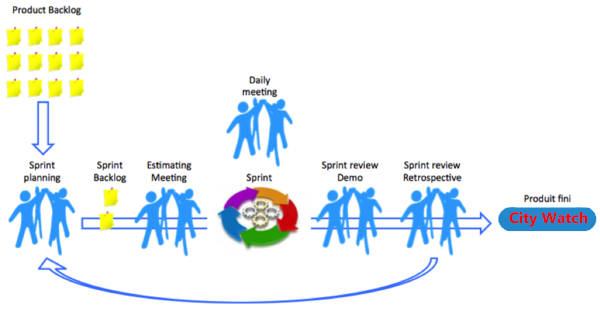
\includegraphics[width=\textwidth]{./figures/scrum-model.tex}
\begin{tikzpicture}

  \node[box]
    (sprints) {Sprints};
  \node[box, left=4em of sprints]
    (planning) {Planning \& System Architecture};
  \node[box, right=4em of sprints]
    (closure) {Closure};

  \draw[->,latex-,line width=0.1em] (5:6em) arc (5:85:6em) node[right=2em] {Wrap};
  \draw[->,latex-,line width=0.1em] (95:6em) node[left=2.5em] {Develop} arc (95:175:6em);
  \draw[->,latex-,line width=0.1em] (185:6em) arc (185:265:6em) node[left=2em] {Adjust};
  \draw[->,latex-,line width=0.1em] (275:6em) node[right=2.5em] {Review} arc (275:355:6em);

  \draw[->,latex-] (planning.west) -- +(-2em,0);
  \draw[->,-latex] (planning.east) to (sprints.west);
  \draw[->,-latex] (sprints.east) to (closure.west);
  \draw[->,-latex] (closure.east) -- +(2em,0);

\end{tikzpicture}
\caption[Méthode Scrum]{La méthode Génie Logiciel Scrum comme décrite par \textcite{Schwaber1995}.}
\captionsource{Daniel G. Siegel, Typical Development Processes of Free and Open Source Software Projects}
\label{fig:scrum-model}
\end{figure}

%\end{document}


\subsubsection{Répartition des rôles}

Chaque projet utilisant la méthode Scrum est monté autour d'une équipe auto-
organisée et multifonctionnelle : auto-organisée car il n'y a pas de chef d'équipe qui
décide les rôles de chacun, ou de la manière dont un problème est résolu, puisque ces
problématiques sont traitées par l'équipe dans son ensemble; et multifonctionnelle car
chaque membre de l'équipe forme une partie prenante dans le développement de
chaque fonctionnalité depuis l'idée jusqu'à l'implémentation finale.
Dans Scrum existe trois principaux rôles:
\begin{itemize}
 \item Le responsable produit (Product owner)
 \item Le Scrum Master
 \item le membre de l'équipe
\end{itemize}

\paragraph{Le responsable produit}

Il prend en charge de communiquer la
vision globale du produit à l'équipe. 
Il se voit représenter le client final, se met à sa place
et priorise ses besoins. Celui qui tient ce rôle est celui qui 
a le plus de visibilité, de responsabilité et d'autorité.
En effet, la méthode Scrum favorise l'auto-organisation de l'équipe.

\paragraph{Le Scrum Master}

Il joue le rôle du communiquant entre le responsable produit et
l'équipe. Il ne gère pas l'équipe, mais veille à éliminer tous les obstacles qui peuvent
empêcher l'équipe d'atteindre les objectifs fixés au cours d'un Sprint. En résumé, ce rôle
permet à l'équipe de rester créative et productive, tout en veillant à ce que les
réalisations soient visibles pour le responsable produit.

\paragraph{L'équipe}

Dans la méthode Scrum, l'équipe est responsable de la réalisation
opérationnelle des Sprints. L'équipe est généralement composée de personnes
multitâches. C'est toute l'équipe qui est responsable du résultat final de chaque sprint.
La manière dont sont exécutées les tâches est très libre mais cette liberté doit être
néanmoins cadrée par l'obligation de répondre aux objectifs du sprint.

\subsubsection{Durées estimées}

Pour montrer l'avancement durant une itération donnée, on a besoin de tracer le
Burndown Chart. Il s'agit d'un graphique simple qui montre le nombre d'heures restant
à effectuer pour finaliser le produit. 

\subsection{Justification du choix de la méthode agile SCRUM}

Aujourd'hui, La méthodes classique présente beaucoup des inconvénients 
\begin{itemize}
 \item Parfois le client a
du mal à exprimer son besoin. Une telle erreur peut s'avérer 
coûteuse d'autant la modification
de certaines fonctionnalités dans le projet n'est pas
tolérée dans la phase de développement.
 \item il est très difficile d'établir dès
le début des paramètres stricts et clairs qui répondent aux attentes du client.
\end{itemize}
Afin éviter ces problèmes, Les caractéristiques de la méthode SCRUM offre
des avantages considérables pour gérer ces problèmes.
\begin{description}
 \item [Personnel engagé] L'une des caractéristiques de SCRUM, 
 c'est que le personnel participe activement à la définition des activités et
 des horaires, de sorte que le degré d'engagement et la motivation sont plus élevés.
 \item [Meilleur vue d'ensemble du projet] Avec SCRUM, les projets 
 précédemment vus dans leur globalité et de façon homogène uniquement par
 les gestionnaires de projets sont désormais accessibles à tous les membres de
 l'équipe de livraison.
 \item [Réduction des bugs] La méthode SCRUM privilégie la qualité et la
 fonctionnalité des développements. Le nombre de bugs et
 de reprises est ainsi réduit.
 \item [Mise à jour des priorité] Au début, le client ignore toute 
 la portée de l'application, ainsi que la façon dont cela pourrait changer avec 
 le temps. Grâce à SCRUM, le client bénéficie d'une flexibilité 
 au niveau de la définition, de l'évolution des priorités et des séquences d'activités.
 \item [Qualité du produit mise en avant] La méthode SCRUM se concentre davantage 
 sur la fourniture d'un service de valeur au client plutôt que sur 
 une date limite fixée.
\end{description}

Scrum est la méthode idéale pour le cas d'une petite équipe et le fait d'avoir un grand 
projet réparti entre cette équipe et aussi il est paraît la meilleure solution pour 
répondre aux exigences du client et réduire la complexité croissante de 
certains projets.

\subsection{Conclusion}

Cette partie nous a permis de présenter le contexte général de notre projet ainsi que la
méthodologie de développement que nous allons adopter
